% ============================================================
% §1.5 Electric Network Interpretation
% ============================================================

\section{Electric Network Interpretation}

\begin{frame}{Electric Network Interpretation}
    % \textbf{Terminology:}
    \begin{description}
        \item[Network] Nodes (vertices) $V$ and conductors (edges) with conductance (edge weight) $C$
        \item[Resistance]  Reciprocal of conductance $R= 1/C$
        \item[Energy] Voltage applied to nodes results in electric energy
        \begin{align*}
            E(u) &= \sum_{x\sim y} C_{xy} \abs{u(x) - u(y)}^{2} && (u:V \to \R)
        \end{align*}
        \item[Restriction] Only apply voltage to \emph{some} nodes $V^{\prime}$ and let others settle into value \note{According to laws of physics the function $u$ will minimize Energy}
    \end{description}

    \vfill
   
  \textbf{Familiar rules:}
  \begin{center}
    \begin{tabular}{c|c}
      Resistors in series     & Resistors in parallel  \\[1ex] \hline
      \begin{tikzpicture}
        [node/.style={draw,circle,inner sep=0mm,minimum size=2mm}]
        
        \node[node, fill=red] (X) [label=below:$x$] {};
        \node[node] (Y) [right=of X, label=below:$y$] {}
        % edge node[auto, swap] {$R_{xy}$} (X);
        edge node[auto, swap] {$R_{1}$} (X);
        \node[node, fill=red] (Z) [right=of Y, label=below:$z$] {}
        % edge node[auto, swap] {$R_{yz}$} (Y);
        edge node[auto, swap] {$R_{2}$} (Y);
      \end{tikzpicture}
                              & \begin{tikzpicture}
                                [node/.style={draw,circle,inner sep=0mm,minimum size=2mm}]
                                
                                \node[node, fill=red] (X) [label=below:$x$] {};
                                \node[node, fill=red] (Y) [right=of X, label=below:$y$] {}
                                edge[bend right] node[auto, swap] {$R_{1}$} (X)
                                edge[bend left] node[auto] {$R_{2}$} (X);
                              \end{tikzpicture}
      \\[1ex] \hline
      % $R_{xz}=R_{xy}+R_{yz}$ & $\frac{1}{R_{xy}} = \frac{1}{R_{1}} + \frac{1}{R_{2}}$
      $R_{xz}=R_{1}+R_{2}$ & $\frac{1}{R_{xy}} = \frac{1}{R_{1}} + \frac{1}{R_{2}}$  
    \end{tabular}
  \end{center}
  
\end{frame}

\begin{frame}{\dwt}
    \textbf{Claim.} Resistance equivalent networks:

    \begin{columns}[c]            % Cols are center vertically aligned
        \begin{column}{.45\textwidth}
            \begin{tikzpicture}
            % [node/.style={draw,circle,inner sep=0mm,minimum size=2mm}]
            [node/.style={draw,fill=black,circle,inner sep=0mm,minimum size=2mm}]
      
            \node[node] (Z) [label=above:$z$] {};
            \node (W) [below=of Z] {}; 
            \node[node, fill=red] (X) [below left=of W, label=below left:$x$] {}
            edge node[auto] {$R$} (Z);
            \node[node, fill=red] (Y) [below right=of W, label=below right:$y$] {}
            edge node[auto, swap] {$R$} (Z)
            edge node[auto] {$R$} (X);;
            \end{tikzpicture}
        \end{column}
        \begin{column}{.45\textwidth}
            \begin{tikzpicture}
            [node/.style={draw,fill=black,circle,inner sep=0mm,minimum size=2mm}]
      
            \node[node] (Z) [label=above:$z$] {};
            \node[node] (W) [below=of Z, label=below:$w$] {}
            edge node[auto, swap] {$R/3$} (Z);
            \node[node, fill=red] (X) [below left=of W, label=below left:$x$] {}
            edge node[auto] {$R/3$} (W);
            \node[node, fill=red] (Y) [below right=of W, label=below right:$y$] {}
            edge node[auto,swap] {$R/3$} (W);;
            \end{tikzpicture}
        \end{column} 
    \end{columns}
    \bigskip

    \textbf{Proof.} Combine rules for resistors in series and in parallel:
    \begin{columns}[t]
        \begin{column}{.4\textwidth}
            Left:
            \begin{align*}
                R_{xy} &= \frac{1}{\frac{1}{R} + \frac{1}{2\,R}} = \frac{2\,R}{3}
            \end{align*}  
        \end{column}
        \begin{column}{.4\textwidth}
            Right:
            \begin{align*}
                R_{xy} &= \frac{R}{3} + \frac{R}{3} = \frac{2\,R}{3}
            \end{align*}
        \end{column}
    \end{columns}
    \bigskip
    
    \begin{remark}
        There exists a formula for the general case of unequal resistances.
    \end{remark}
\end{frame}

\begin{frame}{Renormalization Problem}
    Set all resistances equal to 1 and compute resistance equivalent network!
  
    \bigskip

    \textbf{Unit interval:} Apply rule for resistors in series (trivial):
    \begin{center}
        \begin{tikzpicture}
        [node/.style={draw,circle,inner sep=0mm,minimum size=2mm}]
        
        \node (G1) {$\Gamma_{1}$};
        \node[node] (X) [right=of G1] {};
        \node[node] (Y) [right=of X] {}
        edge node[auto, swap] {$1$} (X);
        \node[node] (Z) [right=of Y] {}
        edge node[auto, swap] {$1$} (Y);
        
        \node (G0) [below=of G1] {$\Gamma_{0}$};
        \node[node] (XX) [right=of G0] {};
        \node (YY) [right=of XX] {};
        \node[node] (ZZ) [right=of YY] {}
        edge node[auto, swap] {$2$} (XX);
        \end{tikzpicture}
    \end{center}
    
    Hence renormalization factor $r=\frac{1}{2}$.   

  
\end{frame}

\begin{frame}
  % TODO: Add resistances to edges
  
  \frametitle{Renormalization Problem II}
  \textbf{SG:}
  \begin{columns}
    \begin{column}{.3\textwidth}
      \begin{figure}
        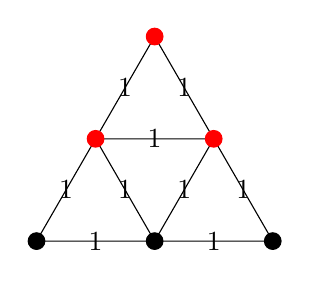
\begin{tikzpicture}[scale=3]
          \draw (0,0) -- node{1} (.5,0) -- node{1} (1,0) -- node{1} (.75,.433) -- node{1} (0.5,0.866) -- node{1} (.25,.433) -- node{1} (0,0);
          \draw (0.5,0) -- node{1} (0.25,0.433) -- node{1} (0.75,0.433) -- node{1} (0.5,0);
          
          \filldraw [black] (0,0) circle (1pt) ;
          \filldraw [black] (1,0) circle (1pt);
          \filldraw [red] (0.5,0.866) circle (1pt);
          \filldraw [black] (0.5,0) circle (1pt);
          \filldraw [red] (0.25,0.433) circle (1pt);
          \filldraw [red] (0.75,0.433) circle (1pt);
        \end{tikzpicture}\\
        \centering
      \end{figure}
      
    \end{column}
    \begin{column}{.3\textwidth}
      \begin{figure}
        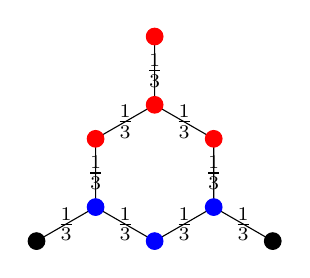
\begin{tikzpicture}[scale=3]
          \draw (0,0) -- node{$\frac{1}{3}$} (.25,.144) -- node{$\frac{1}{3}$} (.25,.433) -- node{$\frac{1}{3}$} (.5,.577);
          \draw (.5,.866) -- node{$\frac{1}{3}$} (.5,.577) -- node{$\frac{1}{3}$} (.75,.433) -- node{$\frac{1}{3}$} (.75,.144);
          \draw (.25,.144) -- node{$\frac{1}{3}$} (.5,.0) -- node{$\frac{1}{3}$} (.75,.144) -- node{$\frac{1}{3}$} (1.0,.0);

          \filldraw [black] (0,0) circle (1pt);
          \filldraw [black] (1,0) circle (1pt);
          \filldraw [red] (0.5,0.866) circle (1pt);
          \filldraw [blue] (0.5,0) circle (1pt);
          \filldraw [red] (0.25,0.433) circle (1pt);
          \filldraw [red] (0.75,0.433) circle (1pt);
          \filldraw [blue] (0.25,0.144) circle (1pt);
          \filldraw [blue] (0.75,0.144) circle (1pt);
          \filldraw [red] (0.5,0.577) circle (1pt);
        \end{tikzpicture}\\
        \centering
        % Resistors in series
        
      \end{figure}
      
    \end{column}


    
    \begin{column}{.3\textwidth}
      \begin{figure}
        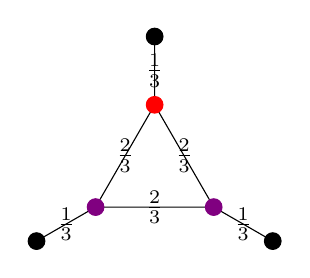
\begin{tikzpicture}[scale=3]
          \draw (0,0) -- node{$\frac{1}{3}$} (.25,.144) -- node{$\frac{2}{3}$} (.5,.577);
          \draw (.5,.866) -- node{$\frac{1}{3}$} (.5,.577) -- node{$\frac{2}{3}$} (.75,.144);
          \draw (.25,.144) -- node{$\frac{2}{3}$} (.75,.144) -- node{$\frac{1}{3}$} (1.0,.0);
          
          \filldraw [black] (0,0) circle (1pt);
          \filldraw [black] (1,0) circle (1pt);
          \filldraw [black] (0.5,0.866) circle (1pt);
          \filldraw [blue!50!red] (0.25,0.144) circle (1pt);
          \filldraw [blue!50!red] (0.75,0.144) circle (1pt);
          \filldraw [red] (0.5,0.577) circle (1pt);
         
        \end{tikzpicture}\\
        \centering
        % \dwt
      \end{figure}
      
    \end{column}
    
  \end{columns}


  
  \begin{columns}
    \begin{column}{.3\textwidth}
      \begin{figure}
        \centering
        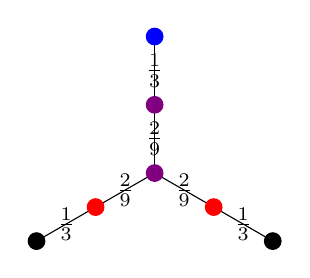
\begin{tikzpicture}[scale=3]
          \draw (0,0) -- node{$\frac{1}{3}$} (.25,.144) -- node{$\frac{2}{9}$} (.5,.288);
          \draw (.5,.866) -- node{$\frac{1}{3}$} (.5,.577) -- node{$\frac{2}{9}$} (.5,.288);
          \draw (.5,.288) --node{$\frac{2}{9}$} (.75,.144) -- node{$\frac{1}{3}$} (1.0,.0);         

          \filldraw [black] (0,0) circle (1pt);
          \filldraw [black] (1,0) circle (1pt);
          \filldraw [blue] (0.5,0.866) circle (1pt);

          \filldraw [red] (0.25,0.144) circle (1pt);
          \filldraw [red] (0.75,0.144) circle (1pt);
          \filldraw [red!50!blue] (0.5,0.577) circle (1pt);
          \filldraw [red!50!blue] (.5,.288) circle (1pt);
        \end{tikzpicture}\\
        % Resistors in series
      \end{figure}
      
    \end{column}

    \begin{column}{.3\textwidth}
      \begin{figure}
        \centering
        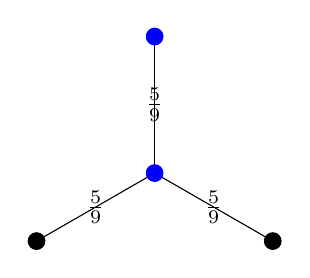
\begin{tikzpicture}[scale=3]         
          \draw (0,0) -- node{$\frac{5}{9}$} (.5,.288);
          \draw (.5,.866)-- node{$\frac{5}{9}$} (.5,.288);
          \draw (.5,.288) -- node{$\frac{5}{9}$} (1.0,.0);

          \filldraw [black] (0,0) circle (1pt);
          \filldraw [black] (1,0) circle (1pt);
          \filldraw [blue] (0.5,0.866) circle (1pt);

          \filldraw [blue] (.5,.288) circle (1pt);
        \end{tikzpicture}\\
        % \dwt
      \end{figure}
      
    \end{column}

    \begin{column}{.3\textwidth}
      \begin{figure}
        \centering
        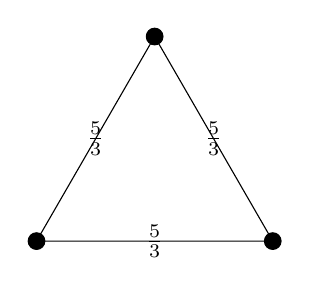
\begin{tikzpicture}[scale=3]
          \filldraw [black] (0,0) circle (1pt);
          \filldraw [black] (1,0) circle (1pt);
          \filldraw [black] (0.5,0.866) circle (1pt);
          
          \draw (.0,.0) -- node{$\frac{5}{3}$} (.5,.866) -- node{$\frac{5}{3}$} (1.0,.0) -- node{$\frac{5}{3}$} (.0,.0);
        \end{tikzpicture}\\
      \end{figure}
      
    \end{column}
  \end{columns}
    \medskip  
    Hence renormalization factor $r=\frac{3}{5}$.

   
\end{frame}




% ============================================================
% §1.6 Effective Resistance Metric
% ============================================================

\section{Effective Resistance Metric}

\begin{frame}[allowframebreaks=.95]{Effective Resistance}
    
    Given a nework, we define the effective resistance between any two points as the resistance between them when restricting to these two points:
    
    \begin{definition}[Effective Resistance]
    Let $x,y \in V$.
        \begin{align*}
            R(x,y)^{-1} := \min \left\{ \E(u) \,\middle\vert\, u(x)=0 \text{ and } u(y)=1 \right\} 
        \end{align*}
    \end{definition}
    \bigskip

    \textbf{Claim.} Equivalent: Minimum value for $R$ such that
    \begin{align*}
        \abs{u(x) - u(y)}^{2} &\leq R\, \E(u) && \text{for all } u \in \dom{\E}.
    \end{align*}
    \bigskip
    \newpage
    
    \textbf{Proof.} Let $u\in \dom{\E}$ such that $u(x)=0$ and $u(y)=1$ and $u$ minimizes $\E(u)$. Thus
    \begin{align*}
        1 = \abs{u(x) - u(y)}^{2} \leq R\, \E(u) = \frac{R}{R(x,y)}
    \end{align*}
    yields $R(x,y) \leq R$.

    For arbitrary $u \in \dom{\E}$ with $u(x) \neq u(y)$ denote $v := \frac{u - u(x)}{u(y)-u(x)}$.
    \note{If u such that u(x) \neq u(y) does not exist the claim is trivial.}
    Then $v(x)=0$ and $v(y)=1$ and
    \begin{align*}
        R(x,y)^{-1} \leq \E(v) = \frac{\E(u)}{\abs{u(x)-u(y)}^{2}}
    \end{align*}
    yields $\abs{u(x)-u(y)}^{2} \leq R(x,y)\,\E(u)$ and therefore $R \leq R(x,y)$.
\end{frame}

\begin{frame}{Effective Resistance on Unit Interval}
  Same as Eucledian distance:
  \begin{itemize}
  \item Function $u$ achieving minimum in definition of eff. resistance is
    harmonic in the complement of $x,y$.  Thus $u$ is the linear
    extension:
    \begin{align*}
      u(t) &=
      \begin{cases}
        0 & t \in [0,x) ,\\
        \frac{t-x}{y-x} & t \in [x,y) ,\\
        1 & t \in [y,1]
      \end{cases} && (\text{assume } x<y).
    \end{align*}
  \item Hence
    \begin{align*}
      \E(u)
      = \int_{0}^{1} \abs{u^{\prime}(t)}^{2} \, \mathrm{d}t
      =\int_{x}^{y}  \frac{1}{(y-x)^{2}} \, \mathrm{d}t
      = \frac{1}{y-x}
    \end{align*}
  \item We obtain
    \begin{align*}
      R(x,y) = \abs{y-x}.
    \end{align*}
  \end{itemize}
  
\end{frame}

\begin{frame}{Effective Resistance is Metric}
    \begin{theorem}[Tower Property]
        Suppose $V^{\prime\prime} \subseteq V^{\prime} \subseteq V$. Given a network on $V$, the restriction to $V^{\prime\prime}$ is equal to the restriction $V^{\prime\prime}$ of the restrction to $V^{\prime}$.
    \end{theorem}
    \bigskip
    
    \textbf{Claim.} Effective resistance fullfills triangle inequality.
    \bigskip

    \textbf{Proof.} Only need to consider $\Delta$-shaped networks. Combine rules for resistors in series and in parallel:

    \begin{columns}[c]
        \begin{column}{.7\textwidth}
            \begin{align*}
                R(x,y) &= \frac{1}{\frac{1}{R_{xy}} + \frac{1}{R_{yz} + R_{zx}}}
                = \frac{R_{xy}\,(R_{yz} + R_{zx})}{R_{xy} + R_{yz} + R_{zx}}
            \end{align*}
        \end{column}

        \begin{column}{.2\textwidth}
            \centering
            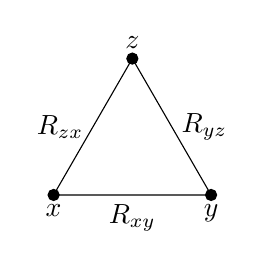
\begin{tikzpicture}[scale=2]
                \filldraw[black] (0,0) circle (1pt) node[below]{$x$};
                \filldraw[black] (1,0) circle (1pt) node[below]{$y$};
                \filldraw[black] (.5,.866) circle (1pt) node[above]{$z$};

               \draw (0,0)
                -- node[below]{$R_{xy}$} (1,0)
                -- node[right]{$R_{yz}$} (.5,.866)
                -- node[left]{$R_{zx}$} (0,0);
            \end{tikzpicture}
        \end{column}
    \end{columns}
    
    Short computation shows
    \begin{align*}
        R(x,y) + R(y,z) = R(z,x) + \frac{2\, R_{xy}\, R_{yz}}{R_{xy} + R_{yz} + R_{zx}} \geq R(z,x).
    \end{align*}   
\end{frame}

\begin{frame}[allowframebreaks]{Effective Resistance on SG}
    \note{Computing effective resistance is complicated. We can give estimates.}

    %\textbf{Aim:} Estimates for $R$.

    \begin{itemize}
        \item Consider neighboring vertices $x,y \in V_{m}$.

        \item Chose $u=\psi^{m}_{y}$ as piecewise harmonic spline, i.e. $\psi^{m}_{y}(z) = \delta_{yz}$ for all $z\in V_{m}$. Then
        \begin{align*}
            \E(u) = \E_{m}(u) = r^{-m}\, E_{m}(u) = r^{-m}\, \sum_{x\sim_m y} \abs{u(x) - u(y)}^{2} \leq 4\,r^{-m}.
        \end{align*}
        \note{Node $y$ has at most 4 neighbors.}
        Hence $R(x,y)^{-1} \leq \E(u) \leq 4\,r^{-m}$.
        
        \item $u(x)=0$ and $u(y)=1$ implies
        \begin{align*}
        \E(u) \geq \E_{m}(u) = r^{-m}\, E_{m}(u) \geq r^{-m}\, \abs{u(x) - u(y)}^{2} = r^{-m}.
        \end{align*}
        \item Conclude
        \begin{align*}
            r^{-m}\leq R(x,y)^{-1} \leq 4\, r^{-m}.
        \end{align*}
        \note{Remember definition of $R(x,y)$.}
        Thus $R(x,y) \sim r^{m}$.
    \end{itemize}
    \newpage
    
    Expansion to other points is possible:
    \begin{theorem}[Estimates for R]
        There exist $C_{1}, C_{2} > 0$ such that
        \begin{enumerate}[(a)]
            \item if $x,y$ are in the same or adjecent $m$-cells
            \begin{align*}
                R(x,y) \leq C_{1}\,r^{m}.
            \end{align*}
            \item if $x,y$ are \emph{not} in the same or adjecent $m$-cells
            \begin{align*}
                R(x,y) \geq C_{2}\,r^{m}.
            \end{align*}
        \end{enumerate}
    \end{theorem}
    \newpage

    \note{$x,y$ are neighbors again.}
    Consider SG on equilateral triangle with edge length 1 and neighboring vertices $x,y \in V_{m}$:
    \begin{itemize}
        \item $\abs{x-y}=2^{-m} = \exp(m\, \log{1/2}) \quad\implies\quad m = \frac{\log\abs{x-y}}{\log{1/2}}$.
        \item Obtain
        \begin{align*}
            r^{m} = \exp(m\, \log{r})
            = \exp\left( \frac{\log\abs{x-y}}{\log{1/2}} \, \log{r} \right)
            =: \abs{x-y}^{\beta}
        \end{align*}
        with
        \begin{align*}
            \beta = \frac{\log{r}}{\log{1/2}}
            = \frac{-\log{1/r}}{-\log{2}}
            = \frac{\log{5/3}}{\log{2}}
        \end{align*}
        \note{$r = \frac{3}{5}$.}
        \item Thus
        \begin{align*}
            R(x,y) &\sim \abs{x-y}^{\beta} && \text{with } \beta < 1.
        \end{align*}
        \item Effective resistance and Euclidian metric are topologically equivalent but they are not equivalent metrics.
        \note{Since $\beta < 1$ (small) distances in resistance metric are much larger than in Euclidean metric.}
    \end{itemize}
\end{frame}


%%% Local Variables:
%%% mode: latex
%%% TeX-master: "./main"
%%% ispell-local-dictionary: "american"
%%% End: